\documentclass[journal,twocolumn]{IEEEtran}
% documentclass[journal, twocolumn]{IEEEtran}
\usepackage{amsfonts}
\usepackage{amsmath,amssymb}
\usepackage{acronym}  % make an acronym
\usepackage{algorithm}
\usepackage{algorithmic}
% \usepackage{balance}
\usepackage{bm}
\usepackage{bbm}
\usepackage{booktabs}
\usepackage{color, soul}
\usepackage{cite}
% \usepackage{flushend}	% Kunzan leads to problems. 
\usepackage{graphicx}
\usepackage{indentfirst}
\usepackage{lipsum}
\usepackage{setspace}
\usepackage{tikz}
\usetikzlibrary{arrows}
\usepackage{subfigure}
\usepackage[amsmath,thmmarks]{ntheorem}
\usepackage{theorem}
% Enable Hyper-references.
\usepackage{hyperref}
\hypersetup{hidelinks, 
colorlinks=true,
allcolors=black,
pdfstartview=Fit,
breaklinks=true}

\def \H {^H}
\def \opt {^{\text{opt}}}
\def \v {\bm v}
\def \w {\bm w}
\def \g {\bm g}
\def \f {\bm f}
\def \T {\bm \Theta}
\def \t {\bm \theta}
\def \x {\bm \xi}
\def \Pmax {P_{\text{max}}}
\def \ml {multi-layer }
\def \tb {transmit beamformer }
\def \sl {single-layer }
\def \diag {\text{diag}}
\def \opt {^{\text{opt}}}
\def \exp {\text{exp}}
\def \arg {\text{arg}}
\def \CN {\mathcal{CN}}
\def \VM {\mathcal{VM}}
\def \re {\text{Re}}
\def \nc {\mathcal{NC}}
\newcommand{\red}[1]{\textcolor{red}{#1}}
\newcommand{\blue}[1]{\textcolor{blue}{#1}}

\begin{document}

\title{Electromagnetic Information Theory: Fundamentals, Modeling, Applications and Open Problems}

% \author{{Jieao~Zhu, Kunzan~Liu, Zhongzhichao~Wan, and Linglong~Dai, {\textit{Fellow, IEEE}}
% }
\author{{Awesome Authors}
\thanks{J. Zhu, Z. Wan, and L. Dai are with the Beijing National Research Center for Information Science and Technology (BNRist) as well as the Department of Electronic Engineering, Tsinghua University, Beijing 100084, China (e-mails: \{zja21, wzzc20\}@mails.tsinghua.edu.cn, daill@tsinghua.edu.cn).


This work was supported in part by the National Key Research and Development Program of China (Grant No.2020YFB1807201), in part by the National Natural Science Foundation of China (Grant No. 62031019), and in part by the European Commission through the H2020-MSCA-ITN META WIRELESS Research Project (Grant No. 956256).}
}

\maketitle

\begin{abstract}
   Massive amount of multiplexing techniques have been proposed to realize the ultra-high-speed wireless communication. These techniques are actually the division of the whole physical resources on a specific perspective. To build a unified theory that can explore the fundamental physical limit of system performance, we should restore to the physical nature of the system. Therefore, electromagnetic information theory (EIT) which analyzes the information conveyed by the continuous electromagnetic field becomes essential. In this article, we systematically investigate the basics and results of EIT. Firstly, we summarize the fundamental analyzing tools of EIT from classical information theory and electromagnetic theory. Then we show the main research content and the corresponding results of EIT, including the continuous modeling, DoF, mutual information and capacity analysis. Finally, we point out several open problems in EIT, based on which further works can be done to improve EIT towards a unified theory.
\end{abstract}

\begin{IEEEkeywords}
    Electromagnetic information theory (EIT), prolate spheroidal wave functions. 
\end{IEEEkeywords}

\section{Introduction}
%% leading paragraph. 
Ultra-high-speed wireless communication are expected to play a cornerstone role in future applications including immersive virtual reality, digital twins, and holographic videos \cite{saad2019vision}. 
In order to fulfill these visions, massive amount of multiplexing technologies have been proposed to exploit various communication resources in the space (SDMA), frequency (FDMA), time (TDMA), polarization, code (CDMA), and even power domains (NOMA) for increasing overall transmission rate. 
Thus, a natural question arises: {\it what is the fundamental physical limit of such multiplexing in a wireless system?}
To answer this question, an intuitive observation is that most of these communication resources correspond to some physical quantities that can be independently manipulated. To be concrete, these quantities are the space, frequency, time, and polarization of an electromagnetic impulse that can be generated and transmitted \cite{shah2022survey}. Though some of these multiplexing technologies are based on mathematical divisions of the channel (CDMA and NOMA), all these multiplexing capability is essentially provided by the electromagnetic fields that finally carry the information \cite{gruber2008new}. Therefore, it is necessary to construct a theory that can model and analyze the wireless information systems built on continuous electromagnetic fields, which leads to the research on electromagnetic information theory (EIT).

%% The definition of EIT. 
EIT is an interdisciplinary subject that merges deterministic physical theory and statistical mathematical theory to study the transmission mechanism of information via spatially continuous electromagnetic field. 
Specifically, it utilizes the basic laws and conclusions in classical electromagnetic theory and information theory to build the system modeling and performance analysis frameworks that fit the electromagnetic propagation theory for wireless information systems. 

%% Difference between EIT and traditional MIMO theory. 
Since EIT is based on the continuous electromagnetic field, it is different from the traditional models with spatially discrete transceivers. 
For example, single-input single-output (SISO) systems consider a pair of points as the transceivers, and MIMO systems regard discrete point sets in certain spatial region as the transceivers. These traditional system models are abstracts of the real communication systems which convey information by continuous field. Therefore, existing analyzing schemes and tools in traditional spatial discrete system models need to be transferred to the corresponding schemes in continuous spatial fields. 



%% Our contributions.
In this article, we systematically investigate the analyzing techniques and the corresponding results of EIT. The key features of this article can be summarized as follows:
\begin{itemize}
\item{The fundamental analyzing techniques and mathematical tools for EIT, which originate from classical information theory and electromagnetic theory, are introduced separately. Specifically, for information theory, the DoF and channel capacity, which are key performance indicators of wireless systems, can be analyzed by using prolate spheroidal wave functions (PSWFs) and statistical theory. For electromagnetic theory, the mainstream is to use Maxwell's equations to build the deterministic electromagnetic field model. Considering both the classical information theory and electromagnetic theory, random fields are introduced to analyze the statistical characteristics of the continuous electromagnetic field, which enables the performance analysis of EIT. }
\item{Based on the fundamental schemes and tools that can be used in EIT, we further investigate the modeling methods of EIT. The deterministic modeling approach and the stochastic modeling approach of the continuous channel are discussed separately. Moreover, the noise model in EIT is built by distinguishing different sources of noise and analyzing the spatial correlation of the noise field. After discussing the model of EIT, DoF, mutual information, and capacity are analyzed by the tools including the PSWFs.} 
\item{Several open problems in EIT are pointed out. For example, the noise model in traditional discrete communication systems and continuous communication systems need to be built compatible, which is a key factor to unify the theory of traditional MIMO systems and continuous systems based on EIT.}
\end{itemize}

\section{Fundamentals}
In this section, we first distinguish between two different definitions of degrees of freedom (DoF) in information theory, where PSWFs are introduced as basic analytical tools to obtain the DoF. 
Then, we clarify the concept of channel capacity and its relation to DoF. 
After that, we introduce Maxwell's equations to describe information transmission via electromagnetic fields. 
Finally, we employ random fields to unify the probabilistic information theory and deterministic field theory. 

% In this section, we will first brief on the fundamental building blocks of the classical one-dimensional time-domain information theory in Subsection~\ref{Sec_2_Subsec_1}. 
% Then, the four-dimensional electromagnetic basics for wireless communications are introduced in Subsection~\ref{Sec_2_Subsec_2}. Finally, two different approaches of combining the information theory with the electromagnetic theory are discussed. 


\subsection{Degrees of Freedom and the Prolate Spheroidal Wave Functions}
\label{Sec_2_Subsec_1}
% introduce the channel DoF. 
The number of degrees of freedom (DoF) is a mathematical quantity that describes how many independent parameters there are in a physical system. 
Usually in the communication context, the DoF refers to the number of orthogonal subchannels that can carry information independently, which is uniquely determined by the channel characteristics and is often calculated by counting the significant singular values of a given channel matrix \cite{goldsmith2003capacity}. 
Thus, we use the term {\textbf{\emph{channel DoF}}} to describe such a number associated with a channel.

% introduce the functional DoF. 
In contrast, the DoF is defined asymptotically in the information theory context. From a rigorous point of view, the (asymptotic) DoF is defined to be the minimum dimension $n$ of a functional subspace $\mathcal{B}_n$ that can approximate any function in a larger space $\mathcal{B}$ with arbitrarily small error $\epsilon$ \cite{poon2005degrees}. For example, the DoF of a $W$-bandlimited signal with observation duration $T$ can be derived by finding the subspace $\mathcal{B}_n$ that contains all the $W$-bandlimited functions that are most concentrated in the time domain. The problem of finding these most concentrated functions, which is named as Slepian's concentration problem, has explicit solutions called PSWFs.
More interestingly, it is proved that in order to approximately represent any function in $\mathcal{B}_W$, it suffices to pick out $2WT+o(2WT)$ PSWFs as basis functions. Thus, the functional DoF of $\mathcal{B}_W$ is $2WT+o(2WT)$ \cite{slepian1976bandwidth}. 
Since this kind of DoF numerically characterizes the possibility to approximate a generally infinite-dimensional functional space $\mathcal{B}$ by a finite-dimensional subspace, we refer to it as the {\textbf{\emph{functional DoF}}}. 
It is worth noting that the functional DoF can be alternatively interpreted as the number of minimal required samples to approximately reconstruct an unknown signal. 

% introduce PSWF and its connection to the evaluation of functional DoF. 
% The explicit evaluation of the functional DoF of arbitrary given functional space is hard in general. However, in some special but important cases this task can be fulfilled by leveraging the constraints that define the functional space.
% For example, the functional space $\mathcal{B}_W$ that contains all the $W$-bandlimited functions can be decomposed by finding those particular bandlimited functions that are most concentrated in the time domain. The problem of finding these most concentrated functions, which is named as Slepian's concentration problem, has explicit solutions called PSWFs.
% More interestingly, it is proved that in order to approximately represent any function in $\mathcal{B}_W$, it suffices to pick out $2WT+o(2WT)$ PSWFs as basis functions. Thus, the functional DoF of $\mathcal{B}_W$ is $2WT+o(2WT)$. 

% Similar to the singular decomposition method for evaluating the channel DoF, the functional DoF of a given signal space is evaluated by approximating the signal space by a finite-dimensional subspace. In the case of band-limited functional space, this decomposition where the basis functions of the subspace are obtained by solving a the Slepian's concentration problem, and the solutions are proved to be the prolate spheroidal wave functions (PSWFs). 

\subsection{Channel Capacity}
\label{Sec_2_Subsec_2}
Different from the notion of channel DoF which characterizes the number of orthogonal subchannels available, the channel capacity measures the error-free information transmission capability of the channel. 
Since the transmission errors are caused by random channel noise, the channel is information-theoretically defined to be a random transfer relationship $p_{Y|X}(y|x)$ with $x$ being the channel input and $y$ being the channel output. 
Then, the mutual information $I(X; Y)$ between a pair of random variables $(X, Y)$ can be defined, and the channel capacity $C$ is defined by taking the supremum of the mutual information over all the input distributions $p_X(\cdot)$ of the channel. Shannon proved in his seminal paper \cite{shannon1948mathematical} that this channel capacity $C$ is ``achievable'' in the sense that for any given error probability $\epsilon$ and code rate $R<C$, there exists a pair of encoder-decoder of sufficient code length that operates below such error probability $\epsilon$. 
Interestingly, he also proved the ``converse'' theorem that for arbitrary code rate $R>C$, no matter what code is employed, the error probability is bounded away from zero, indicating that it is impossible to realize error-free transmission when $R>C$. Thus, the quantity $C$ is established to be the fundamental transmission limit of such a channel $p_{Y|X}$. 


% The second step is to discretize the continuous time-domain waveform channel into a series of independent symbol channels, and sum over the capacities of each symbol channel to obtain the overall waveform channel capacity. Without loss of generality, a $W$-bandlimited waveform channel is first considered, which is equivalent to setting $h(t)=W{\rm sinc}(Wt)$. Not rigorously, this discretization step is done by the Shannon-Nyquist sampling theorem, stating that a number of $2WT$ independent samples can be obtained from a waveform channel bandlimited to $W$ and time-limited to $T$. From a more rigorous functional point of view, the $W$-bandlimited waveform channel is viewed as a projection operator $\mathcal{B}$ that maps a signal $x\in{\mathcal{L}^2(\mathbb{R})}$ into the bandlimited received signal $y={\mathcal{B}x}$, and the information-transmission capability of such operator $\mathcal{B}$ is characterized by its eigenvalues over a finite time interval $[-T/2, T/2]$. This eigenproblem is referred as the Slepian's concentration problem. Solving this eigenproblem directly leads to the eigenfunctions called prolate spheroidal wave functions (PSWF), and the number of significant eigenvalues above a certain threshold is exactly $2WT+\mathcal{O}(\log(WT))$. The number of these dominating eigenvalues are often referred to as the degrees of freedom (DoF) of this channel, which means that this $W$-bandlimited $T$-timelimited waveform channel can be asymptotically viewed as $2WT$ parallel Gaussian symbol channels, as $T\to\infty$. The capacity of a $W$-bandlimited channel, in bits per second, can then be derived accordingly. 

% The third step is to integrate over the frequency axis to get the overall capacity, exploiting the capacity result of a $W$-bandlimited waveform channel. Specifically, for any given small frequency band $[f, f+{\rm d}f]$, the capacity of such infinitesimal sub-channel is jointly determined by the frequency response $|H(j2\pi f)|^2$ of $h(t)$, the AWGN noise level, and the power budget\footnote{The power budget of the transmitted signal $x(t)$ is usually characterized by the power spectral density (PSD) $S_x(f)$, where $f$ varies within the bandwidth of the wireless system in question. } of transmitted signal $S_x(f)$ at single frequency point $f$. Thus, integrating over the entire frequency axis yields a capacity value of the AWGN waveform channel with impulse response $h(t)$. The achievability and converse of such a capacity is guaranteed by performing asymptotic error analysis on all the above three deduction steps. 

\subsection{Electromagnetic Theory}
\label{Sec_2_Subsec_3}
% Basics about electromagnetics.
Electromagnetic theory is a branch of physics that studies the electromagnetic (EM) interaction in four-dimensional spacetime from a field-theoretic point of view. The EM forces are carried by EM vector fields, which are usually described by Maxwell's equations. Maxwell's equations are four linear partial differential equations that characterize how the electric fields and magnetic fields are altered by each other and by charges and currents. Combining these four equations, a vector wave equation can be obtained that manifests the existence of EM waves. 

In wireless communications, in order to describe the EM response at the receiver induced by the transmitted wave at the transmitter, Green's function $\bm G$ is often introduced as the spatial impulse response of the EM system \cite{stratton2007electromagnetic}. Since the electric and magnetic field vectors are all three-dimensional time-varying vectors, Green's function is a dyad-valued function of spacetime. 
Note that EM theory is a deterministic theory built on partial differential equations, and thus Green's function is uniquely determined by the boundary conditions of the EM problem.
As a result, pure EM theory cannot capture the random nature that arises in communications. 

\subsection{Random Fields}
\label{Sec_2_Subsec_4}
In order to apply information-theoretic analysis to EM fields, probabilistic measures should be assigned to the functional space containing all the possible EM fields that satisfy Maxwell's equations, which leads to the random field modeling for EIT. 
Random fields are well-studied mathematical objects, among which the Gaussian random fields (GRFs) are the most widely applied instances. 

GRFs are random multivariate functions whose finite-dimensional marginal distributions are Gaussian. Justified by the central limit theorem, many complicated spatially dependent random values that arise in communications can be modeled by GRFs.  
Inheriting favorable mathematical properties from Gaussian distributions, such GRF modeling exhibits good analytical properties that can facilitate both theoretical deduction and numerical inference. 

In EIT, the GRFs can be utilized to model both the EM channels and the EM signals. Since in real-world communication scenarios the EM channel responses vary randomly as a function of spacetime, it is reasonable to model such spatio-temporal variations by a channel GRF, thus allowing Bayesian inference of the channel entries that are not directly measured. 
Similarly, in order to capture the randomness of the transmitted and received signals, the current distributions $\bm J$ at the transmitter and the electric fields $\bm E$ at the receiver can also be modeled by GRFs \cite{wan2022mutual}, from which information-theoretic quantities $I({\bm J};{\bm E})$ can be defined to characterize the information transmission capability of such EM channel. 
\begin{figure}
	\centering 
	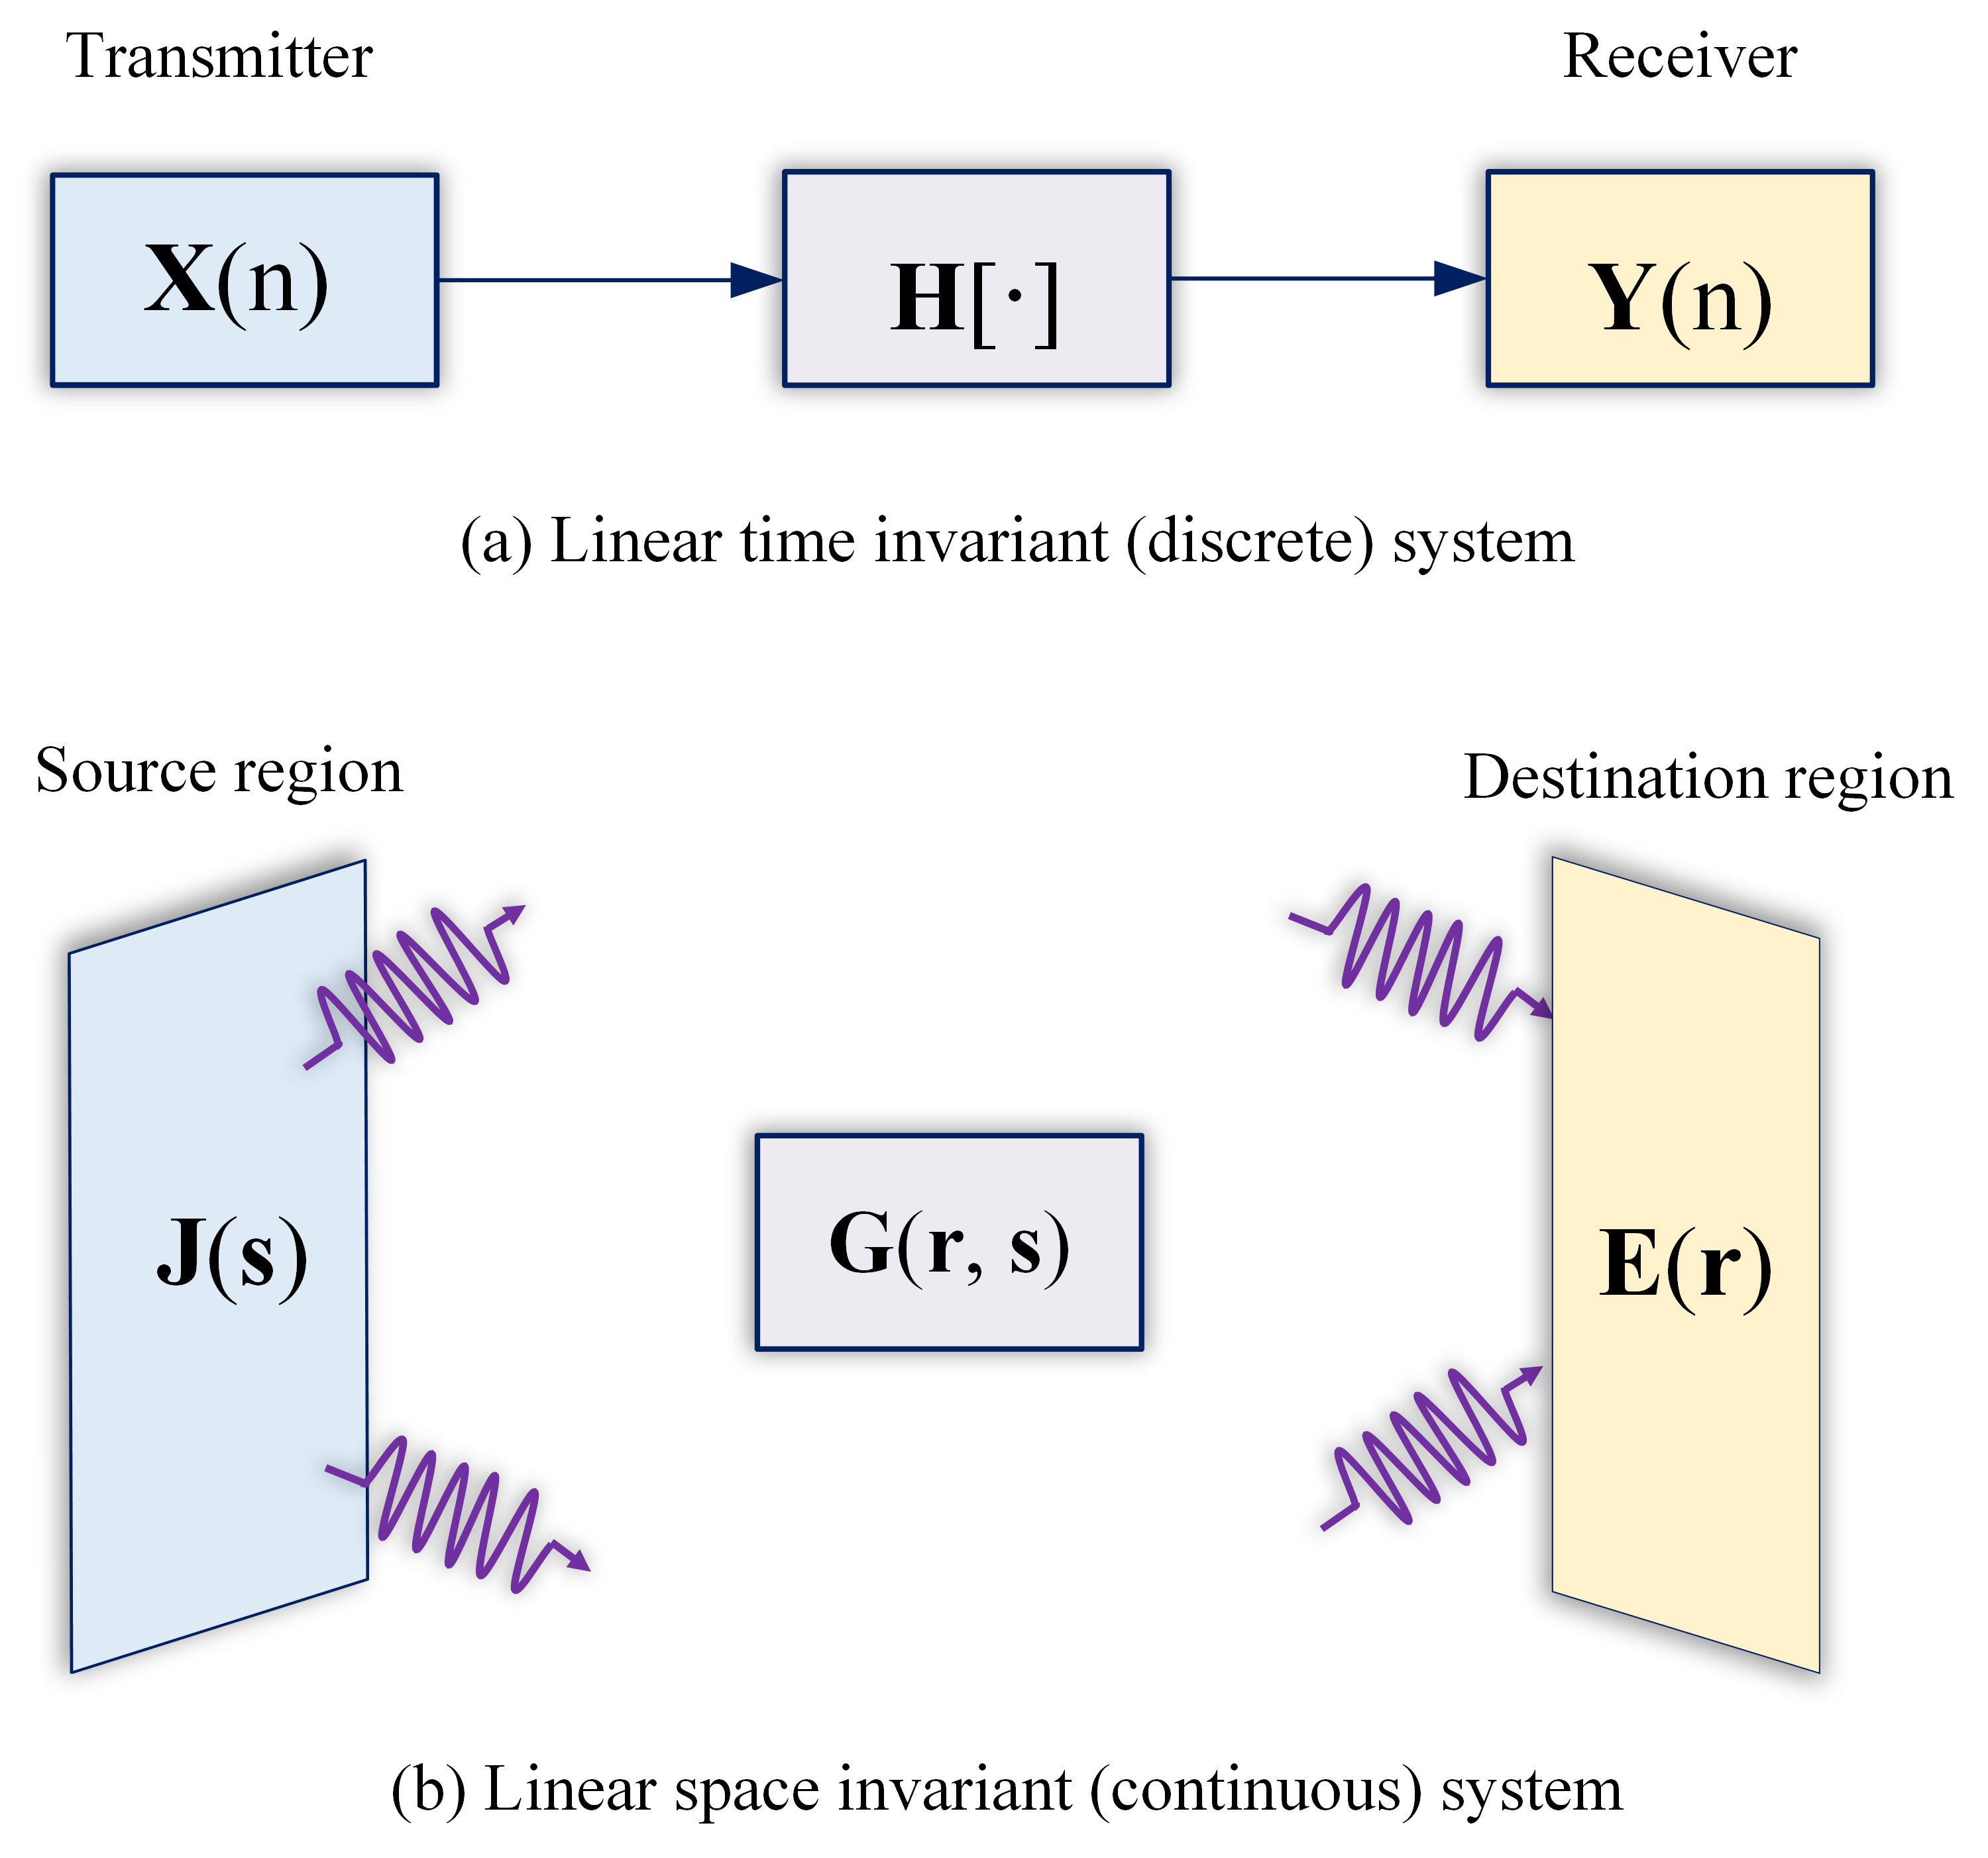
\includegraphics[%height=4cm,
	width=6.8cm]{figures/Shannon_Marzetta.png} 
	\caption{Linear time invariant and linear space invariant systems.} 
	\label{fig:Shabbon_Marzetta}
\end{figure}

% Motivated by the possibility of exploiting the three spatial dimensions, the multi-input multi-output (MIMO) architecture have been ubiquitous in contemporary wireless communication systems. To fully exploit the potential of MIMO, numerous spatial multiplexing technologies have been proposed, including SDMA, TRDMA, PDMA, and LDMA. However, there must be a unified underlying theory that governs all the multiplexing technologies, since they are all based on the same physical media of electromagnetic waves. To construct this unified theory, two different approaches have been proposed in the literature to characterize the electromagnetic channel. 

% The first approach is to model the electromagnetic channel in a deterministic manner. The determination of the modeling means the channel is treated as a fully predictable function of spacetime, as long as the geometric parameters of the transceivers and the scatterers are known. A typical modeling of such a deterministic channel is describing the electromagnetic channel with the dyadic Green's function. The dyadic Green's function, which can be directly derived by solving the vector wave equation of electromagnetic fields, can be regarded as the spatial impulse response of the electromagnetic field with given boundary conditions. Similar to the decomposition of a $W$-bandlimited time-domain waveform channel, the four-dimensional electromagnetic channel, described by some deterministic Green's function, can be decomposed onto a certain orthonormal eigenfunctions, and the corresponding eigenvalue set determines all the information-theoretic numerical characteristics of such channel, including the DoF and capacity.

% The second approach is to model the electromagnetic channel in a stochastic manner. Instead of treating the electromagnetic channel by some deterministic impulse response, this stochastic modeling regards the channel itself as a random field, in which the electromagnetic constraints brought by Maxwell's equations are encoded in the auto-correlation function of such a random field. By this approach, we can obtain the ergodic capacity, but the exact DoF cannot be defined with such a stochastic assumption.  


% In wireless communications, electromagnetic waves are often exploited to carry information by manipulating their amplitudes, frequencies, and phases. To transmit and receive the electromagnetic waves, antennas are designed to radiate the waves into the free space at the transmitter, and couple the waves into electronic circuits at the receiver. Thus, from an end-to-end point of view, by applying antennas, the electromagnetic channel in four-dimensional spacetime is simplified into a time-domain waveform channel with only one temporal dimension. 
% In this simplified model, both the electromagnetic properties of the propagation environment and the detailed design of the antennas are condensed into an end-to-end impulse response $h(t)$ of the time-domain equivalent channel, to which Shannon's information-theoretic approach in the previous Subsection~\ref{Sec_2_Subsec_1} can then be applied. 
% It is worth noting that, with this end-to-end single-input single-output (SISO) model, only one time dimension out of four spacetime dimensions of the electromagnetic waves can be efficiently utilized. Thus, the DoF of the electromagnetic channel is well under-exploited in SISO technology. 


\section{Modeling and Information-Theoretic Analysis}
In this section, we will first discuss the continuous modeling scheme in EIT, which contains the channel modeling and the noise field modeling. Based on the continuous modeling of the system, we further utilize tools in information theory like PSWF to derive the DoF, mutual information and capacity.
\subsection{Continuous Modeling in Electromagnetic Information Theory}
\subsubsection{Continuous channel modeling}
In this part we will discuss the channel models in EIT, which focuses on the linear transformation between the received field and the noiseless radiated field. 
% Since spatial multiplexing can only be realized with MIMO technology, we will always assume a MIMO transceiver in the sequel. 
To model the traditional narrow-band MIMO channel, a matrix with complex-valued entries is usually utilized, each representing the complex channel gain between a pair of transceiver antennas. 
This channel model is, in essence, spatially discrete. 
However, in EIT, it is reasonably assumed that one is able to detect the field at an arbitrary point inside the receiver region, where the precision of such measurement is subject to some physical noise limits, which naturally leads to the assumption that the transceivers operate in a continuum of space.  

This idea of continuous modeling, though seems impossible to have its hardware counterpart in reality, is of both theoretical convenience and practical reasons. 
The theoretical convenience originates from the fact that the fundamental physical laws that rule the electromagnetic phenomena are, intrinsically, continuous and linear. 
As a result, extensive mathematical tools, including functional analysis, linear operator theory, and complex analysis have already been developed to attack these continuous linear problems. 
The practical reasons are that the real-world antenna-based point-to-point transmission models can be viewed as a special case of the continuous model. 
Mathematically, an antenna acts as a continuous integral operator that weights the incident signal by its electromagnetic eigenmode, which corresponds with the continuous modeling in EIT. 
Thus, the EIT channel model is expected to be written in a continuous linear operator language, whether the operator is deterministic or stochastic.
\begin{figure}
	\centering 
	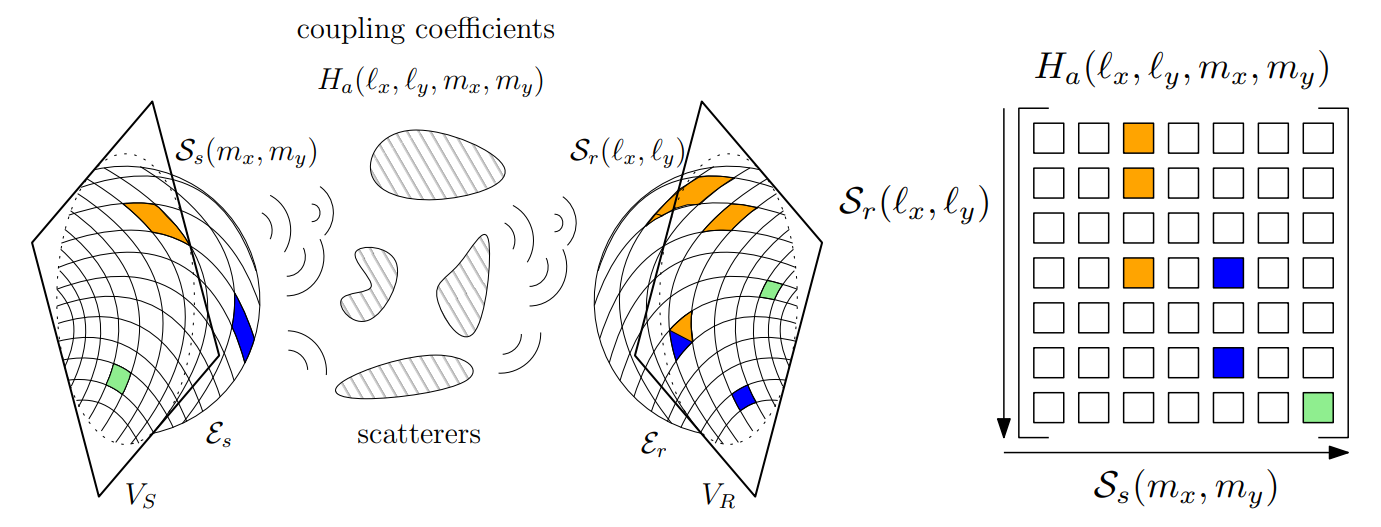
\includegraphics[width=\linewidth]{figures/random_channel.png} 
	\caption{Continuous channel modeling with Fourier plane-wave series expansion \cite{marzetta2022fourier}.} 
	\label{fig:marzetta}
\end{figure}

On the deterministic channel modeling approach, the channel is fixed or at least varying slowly. The simplest deterministic continuous channel model is the line-of-sight (LoS) model, which assumes no scatterers between the transceivers. In this scenario, the operator of the channel is the Green's function in free space. More complex modeling schemes consider the scatterers and classify them into different clusters. The channel operator depends on the location of the clusters.

Another approach which uses stochastic channel model assumes that some given statistical characteristics of the channel can be obtained. As introduced in Subsection~\ref{Sec_2_Subsec_4}, GRFs are suitable to model the randomness of the channel and can provide useful tools such as Bayesian inference for channel estimation. For the stochastic channel modeling, a widely used scheme is the Fourier plane-wave expansion which decomposes the channel using plane waves \cite{marzetta2022fourier}. Such expansion is shown in Fig. \ref{fig:marzetta} and is equal to performing the Fourier transform on the stochastic channel. The spectrum of the channel in the wavenumber domain and the autocorrelation function of the channel can also be derived under the GRF channel model, which can facilitate the mutual information and capacity analysis of the channel.


\subsubsection{Noise field modeling}
After the discussion of the continuous random channel model, we will introduce the noise modeling scheme in this part. In classical information theory, the noise is usually modeled by a time-domain AWGN, since the AWGN has a flat power spectral density (PSD) and,  furthermore, its projection coefficients onto any orthonormal basis are independent and of equal power, which is beneficial to theoretical analysis. 
Similarly, in EIT, the noise is usually modeled by a spatial AWGN with flat wavenumber PSD. This spatial AWGN implies that the additive noises at any small spatial regions are independent and identically distributed (i.i.d) proper complex Gaussian random variables whose variances are proportional to the volume of the small region. This is the simplest noise model in EIT, which is convenient for analysis, but there is still gaps towards the reality. 

In general, the noise values that emerge on different points of space cannot be assumed independent, i.e., they exhibit some spatial correlation. 
This is because the noise is not completely composed of spatially uncorrelated thermal noise. 
The unwanted interference waves also wander in the space and enter the receiver, leading to an equivalent noise signal which are spatially correlated in general. 
To characterize this electromagnetic interference, we borrow the one-ring model from prior works on channel modeling, and extend this model to a more general one-sphere scenario with polarized electromagnetic waves, while the exact expressions of the spatial correlation function can still be obtained. 
This non-white spatially correlated noise model is of theoretical importance, since it is provably compatible with the Maxwell's equations, while other noise models including the sinc-shaped or jinc-shaped correlation functions either fail to satisfy the Maxwell's constraints, or ignore the polarization of the electromagnetic waves. 


\subsection{Functional DoF and Channel DoF}
\label{Sec_3_Subsec_2}
For a wireless system, the degree of freedom (DoF) shows the maximum number of independent channels that can be utilized to transmit information. For example, the degrees of freedom of traditional MIMO system is usually approximated by the minimum value of the number of transmitting antennas and the number of receiving antennas. However, such approximation fails when we consider massive antennas in a spatial-constraint region, because the DoF will tend to infinity with the growth of the number of antennas according to the approximation. Therefore, the DoF of spatially constrained continuous wireless system is worth analyzing. In this part, we will discuss the functional DoF and channel DoF in EIT separately and summarize the related works.

\subsubsection{Functional DoF}
As we have clarified in Section~\ref{Sec_2_Subsec_2}, the functional DoF in classical information theory defines the minimum number of samples that is needed to reconstruct the signal. Similarly, in EIT, the functional DoF refers to the minimum number of samples that is needed to reconstruct a given electromagnetic field. The analysis of such DoF is similar to the Nyquist sampling theorem in classical information theory. If we observe the electromagnetic field in a spatially limited region, of which the size is far greater than the wavelength of the electromagnetic field, then we can perform half-wavelength sampling on the region. The DoF that can be obtained from the region is proportional to its length or area. 

\begin{figure}
	\centering 
	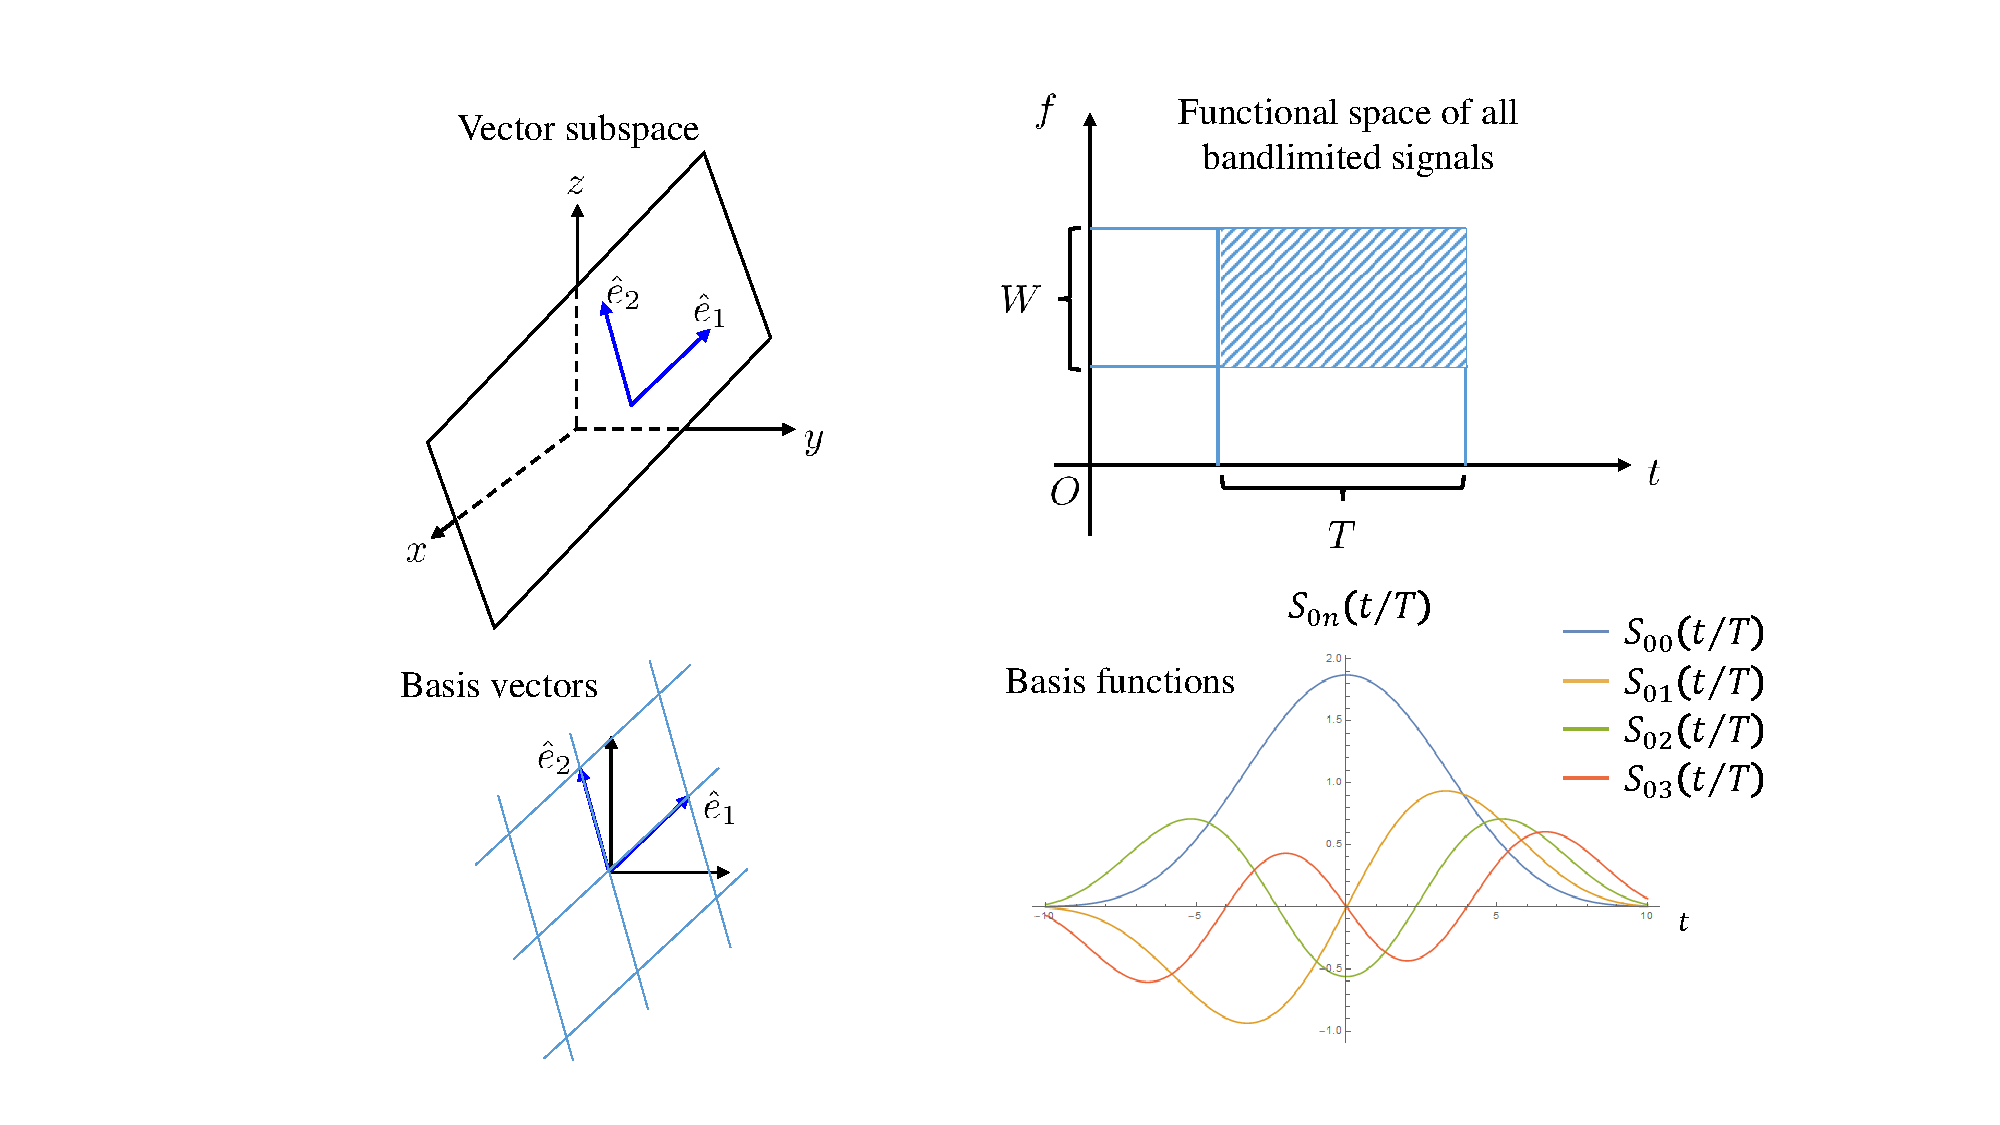
\includegraphics[width=\linewidth]{figures/PSWF.pdf} 
	\caption{Illustration of functional spaces and their analogy with finite-dimensional vector spaces }
	\label{fig:CAPMIMO}
\end{figure}

In the analysis approach of spatial functional DoF, a notion named spatial bandwidth is introduced, which extends the bandwidth in classic information theory to spatial domain. The bandwidth in classic information theory depicts the band-limited characteristics of the signal in the frequency domain, and can be used to derive the DoF of the signal according to Nyquist sampling theorem. Similarly, the spatial bandwidth depicts the band-limited characteristics of the electromagnetic field in the wavenumber domain, and can be used to derive the DoF of the electromagnetic field in the space-wavenumber domain. For a given channel model, the spatial bandwidth can be approximated using the method of steepest descent \cite{bucci1987spatial}. More general results considering the four-dimensional spacetime are based on Landau's eigenvalue problem.

\subsubsection{Channel DoF}
Furthermore, if we consider the wireless communication between two continuous regions in the space, we need to analyze the channel DoF which relies on the channel model and represents the maximum number of independent channels that can be used to transmit information. For line-of-sight (LoS) channel, which is the simplest model that is easy to analyze, the DoF is solved by expanding the continuous channel on a series of orthogonal sub-channels and counting the number of channel gains that exceed a threshold. This procedure can be transferred to solving an eigenvalue problem which utilizes the Hermitian kernel constructed from the channel response. For the LoS channel model, the channel response is Green's function and the eigenvalue problem can be approximated by the Slepian's concentration problem, which utilizes PSWFs to express the eigenfunctions and has been well studied. Through this approach, the DoF of LoS channel model can be well approximated, which is proportional to the product of the area of the transceivers. 

For the DoF analysis in more complicated channel models, especially the scenarios with scatterers between the transceivers, there are two approaches that rely on the channel modeling scheme. 
If the channel is modeled as deterministic channel with known scatterer positions, the clusters can be grouped into several solid angular region and ray-tracing model is applied. 
In this channel modeling approach the solid angles of the scatterer cluster observed from the transceivers actually determine the bandwidth in the wavenumber domain. 
Therefore, the Slepian's concentration problem can also be applied to this scenario and the DoF is proportional to the solid angle of the scatterer cluster and the length of the transceivers. 
If the channel is modeled as stochastic channel with random scatterer positions, uniform distribution, von Mises-Fisher  distribution or other distribution functions can be used to model the statistical characteristics of the channel. 
The DoF of the channel in this model should be the expected value averaged by probability.

% maybe this paragraph is not needed. Put it here temporarily


\subsection{Mutual Information and Capacity Analysis}
Besides the DoF which reveals the available sub-channels that can be used to transmit information, the channel capacity is another important performance indicator, which shows the limit of the information transmission rate of the wireless system. Compared to traditional MIMO information theory which uses random vectors as transmitted and received signals, electromagnetic information theory models the electromagnetic field as random field. The random field modeling follows the statistical approach of mutual information and capacity analysis of Shannon. Each realization of the random field represents a pattern of the radiating field. The ensemble of the realizations, to which a probability measure is assigned, depicts the statistical characteristics of the system. 

The mutual information and capacity analysis based on random field can be viewed as the extension of the corresponding analysis based on random vector. The main difference between them is that the former approach is in the continuous domain and the latter approach is in the discrete domain. For electromagnetic information theory, operator theory can be used to represent the characteristics of the random field. 
Utilizing the KL expansion scheme, the random field can be decomposed to uncorrelated random variables on orthogonal basis. Then the continuous channel can be viewed as the superposition of all the sub-channels. The information that can be obtained from the received random field is then derived by summing the information of all the sub-channels. Utilizing Fredholm determinant which defines the determinant of operator rather than matrix and is widely used in physics, the mutual information between the transmitted field and the received field can be represented by a closed-form formula. Maximizing the mutual information by optimizing the distribution of the random field, the channel capacity of the continuous wireless system can be obtained. 

\section{Applications of the Electromagnetic Information Theory}
In this section, we will introduce several applications of the EIT, which utilize the tools and results of EIT to achieve better performance compared with the state-of-art technologies.
\subsection{Location Division Multiple Access}
\begin{figure*}
	\centering 
	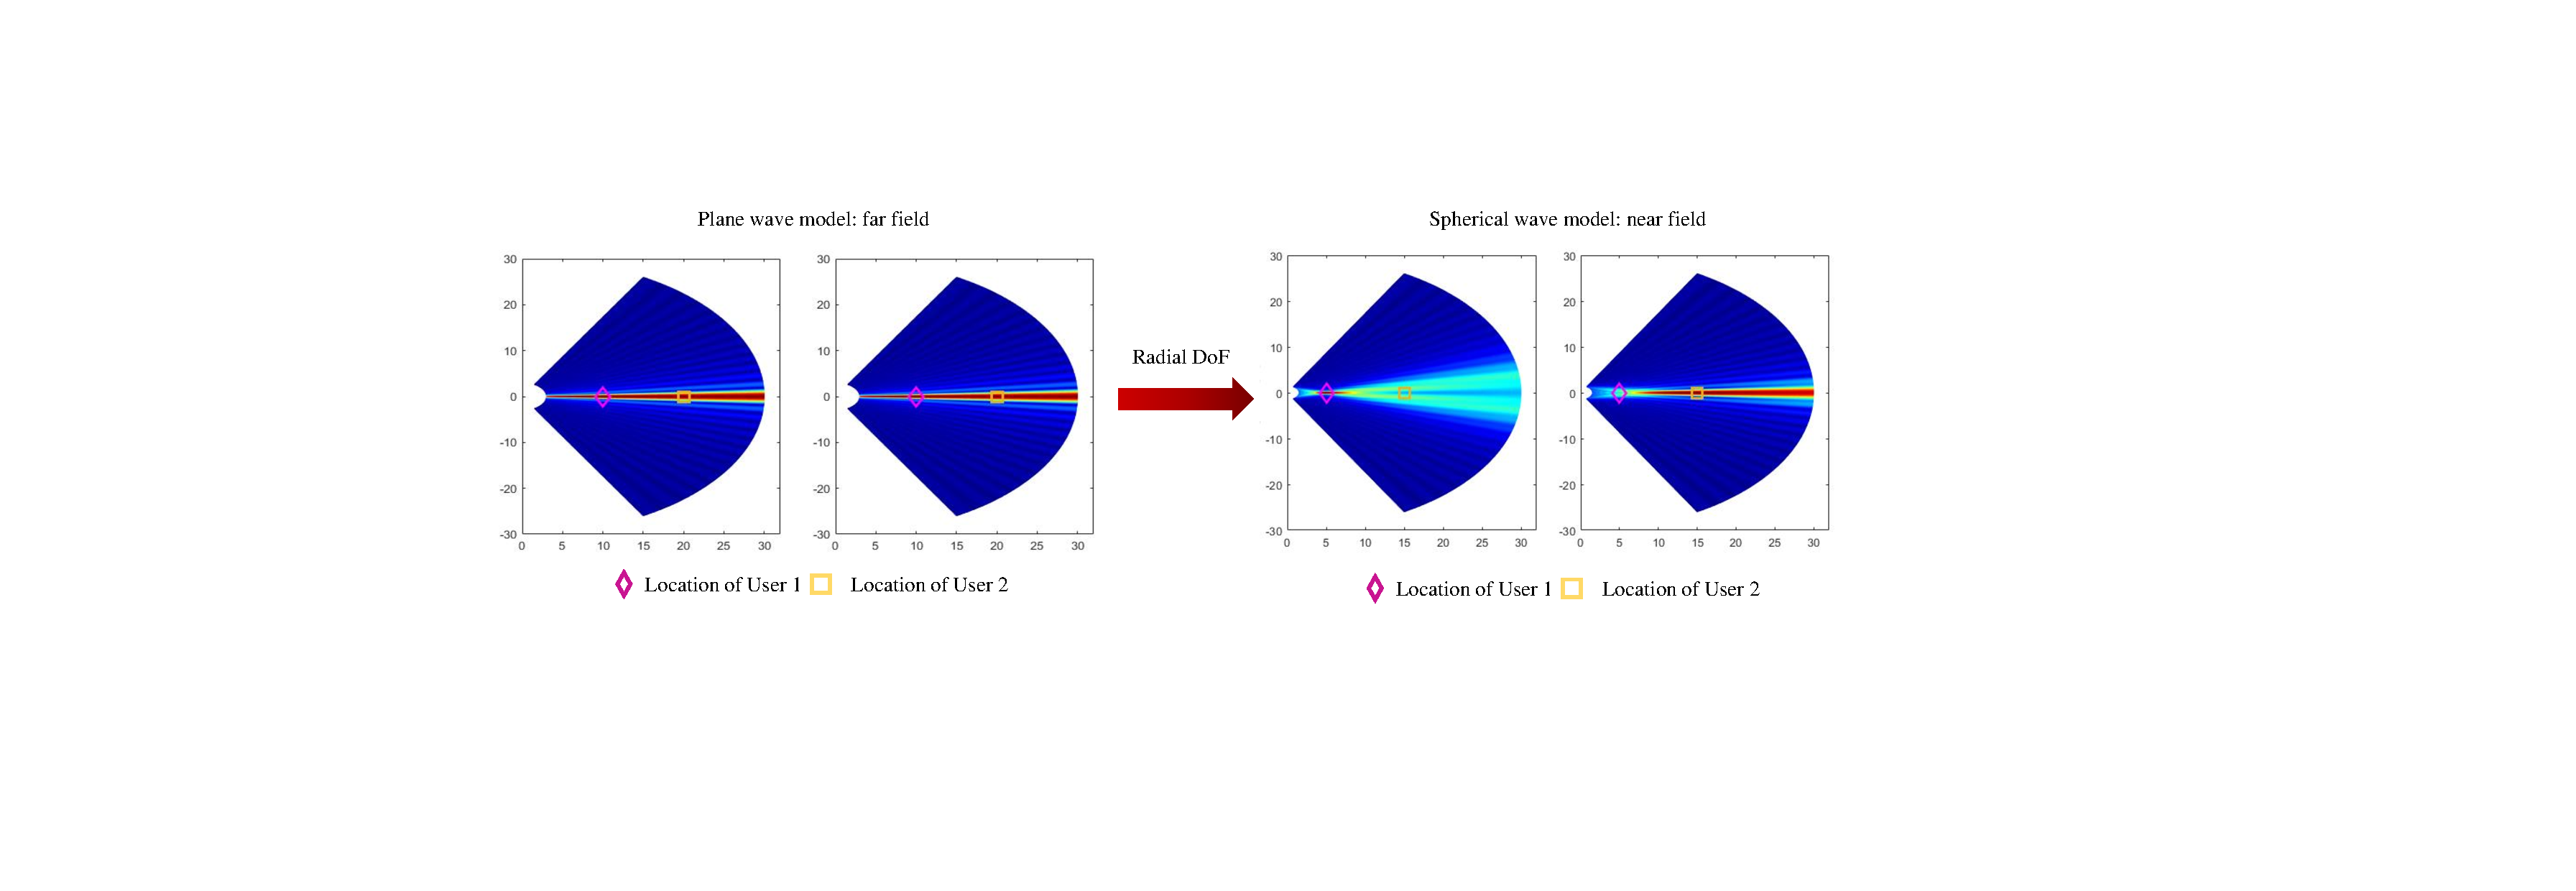
\includegraphics[width=\textwidth]{figures/LDMA.pdf} 
	\caption{Comparison between the SDMA scheme which can not utilize the radial DoF and the LDMA scheme which exploits the radial DoF. \cite{wu2022multiple} }
	\label{fig:LDMA}
\end{figure*}
For multiple access schemes, the beams emitted from the base station form a functional space. The DoF of the functional space represents the resolution of the base station to users at different locations, which corresponds to the analysis of functional DoF in EIT. 
Traditional space-division multiple access based on the far-field model can only distinguish the users by the angles and does not utilize the functional DoF in the radial dimension. 
For the massive MIMO system which adopts a large-scale antenna array, spherical wave model is used instead of the plane wave assumption. 
With the spherical wave model, in addition to the angular dimension, the users can also be distinguished along the radial dimension. 
Therefore, a new division scheme called the location division multiple access (LDMA) is proposed to fully exploit the functional DoF of the beams and serve users at different angles and distances. 
In the LDMA scheme, near-field codebook, beam training and channel estimation are designed correspondingly, aiming at fully utilizing the spatial resources. 

\subsection{Near Field DoF}
As discussed in Subsection~\ref{Sec_3_Subsec_2}, the channel DoF of a LoS channel model in EIT is approximately proportional to the length of the transceivers and inversely proportional to the distance between the transceivers. Therefore, unlike the traditional far-field scenario which can only support one data stream in the LoS channel model, in the near-field region, the wireless communication system has high channel DoF and can support more than one data streams. To fully utilize the near-field channel DoF, a distance-aware precoding scheme is proposed \cite{wu2022multiple}, which adaptively adjusts the number of radio frequency chains to match the channel DoF with different distances.   

% \subsection{Pilot overhead reduction}
% The pilot overhead without channel state information will increase linearly with the number of the antennas. For massive MIMO systems, the pilot overhead will be intolerable. Therefore, to reduce the pilot overhead, the prior information of the channel need to be obtained, which projects the high-dimensional channel matrix on a low-dimensional subspace. Such schemes are actually the expansion of the well-known compressed sensing method, which utilizes the sparsity of the channel. The prior information of the channel can be obtained by building the channel model as a random field and analyzing its statistical characteristics. According to the random channel model, the sparsity of it can be explored to derive the required number of dimensions for channel estimation. 

\subsection{Continuous Aperture MIMO}
Traditional wireless communication systems deploy finite antennas in a limited aperture as the transceivers. To break the performance limit in limited aperture, continuous aperture MIMO (CAP-MIMO), which is also called holographic MIMO, is proposed. CAP-MIMO, which is as the ultimate case of MIMO system, uses a structure that contains infinite dense antennas in a limited spatial region. Such structure equals to continuous apertures that can generate arbitrary current on the transmitter side and detect any electric field on the receiver side. The current distributions on the transmitter are called patterns of the CAP-MIMO. Different signals are modulated on the patterns separately and radiated to the space. Designing the patterns are actually designing the channel division scheme, thus is key to the performance of the CAP-MIMO system \cite{zhang2022pdma}.

\begin{figure*}
	\centering 
	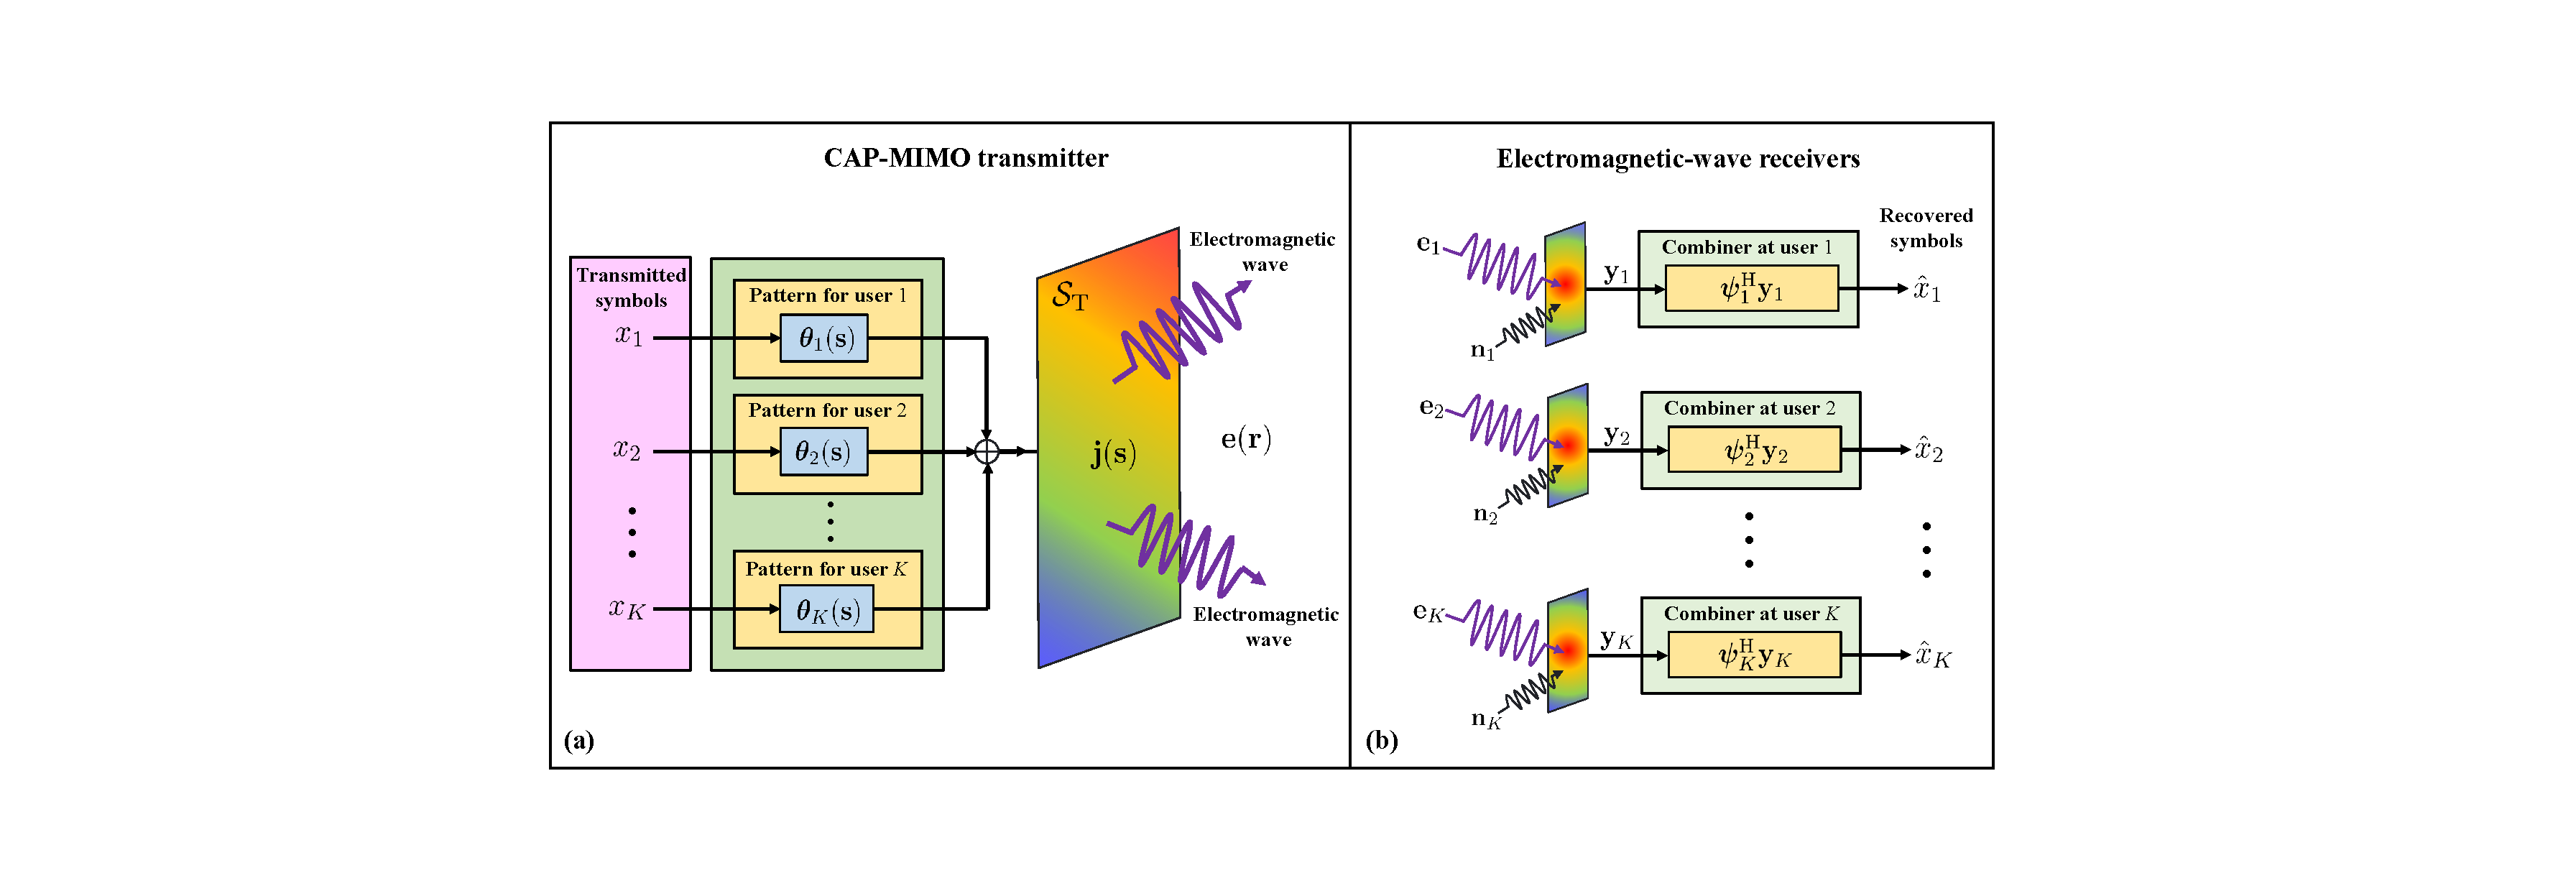
\includegraphics[height=8cm, width=15cm]{figures/CAPMIMO.pdf} 
	\caption{Illustration of CAP-MIMO transceivers \cite{zhang2022pdma} }
	\label{fig:CAPMIMO}
\end{figure*}

% Several works have already explored the pattern design scheme for CAP-MIMO system. The simplest and the easiest way to implement is utilizing the Fourier basis as the patterns, which transfer the approach of OFDM scheme in the time-frequency domain to spatial-wavenumber domain. Other special functions are also utilized to design the patterns in the corresponding assumptions like line-of sight communication or single receiver. For general scenarios, the continuous current patterns can be projected to orthogonal basis and optimization schemes can be utilized to obtain the near-optimal solution of the pattern design scheme.

\subsection{Field Reconstruction}
In engineering practice, it is often required to reconstruct the values of an electromagnetic field from a finite number of available observations, which is called the field reconstruction problem. 
To solve this problem, prior information about the electromagnetic field is often exploited, including the spatially band-limited property and the spatial correlation that the electromagnetic field exhibits. 
The spatially bandlimited property justifies the cardinal series $\sum_n e(n{\bm Q}) {\rm jinc}(|{\bm r}-n{\bm Q}|)$ as asymptotically optimal linear interpolators \cite{pizzo2022nyquist} of the electromagnetic field, while the field correlation function leads to Gaussian process regression (GPR)-based field interpolators. 
These field interpolators have wide applications in field measurement tasks and channel prediction problems. 

\section{Open Problems}
In this section, we will enumerate some open problems related to EIT, including how to construct a physically compatible noise model, how to specify the power constraint of a continuous-aperture transmitter, how to prove the achievability of the EIT capacity, and what is the fundamental physical limit of manipulating a current density on a continuous transmitting aperture. 

\subsection{Compatible Noise Modeling in Discrete and Continuous Communication Systems}
It can be proved that a purely i.i.d. thermal noise distribution will cause the divergence of the end-to-end capacity of a MIMO transceiver within a constrained aperture size in EIT, as the number of receiving antennas $N$ increases and finally approaches the continuous case. 
This is because, as the number of receiving antennas increases, the signals can be aggregated coherently within any small spatial region, while the noises add up out-of-phase because of their uncorrelatedness. 
Thus, in this small region the signal energy scales as $\mathcal{O}(N^2)$, while the noise energy scales as $\mathcal{O}(N)$, leading to an $N$-fold improvement of SNR. As $N\to\infty$, the capacity will diverge to infinity, which is obviously impossible.  

This absurdity is, in fact, caused by the improper assumption that the noise is spatially uncorrelated. If we assume a correlated noise, which is possibly the actual correct model, then this capacity divergence naturally disappears. 
Thus, a correlated noise model is needed for the capacity analysis of EIT. This model may be tuned to exhibit a small enough spatial ``coherence length'' to be compatible with the independent  MIMO noise model with $\lambda/2$-spaced antennas, while it does possess some spatial correlation in a small scale to ensure a finite-valued EIT capacity. 
The construction of such a kind of noise model that bridges the macro-scale and micro-scale noises is, up to date, an open problem. 

\subsection{Power Constraint of the Continuous Communication System}
For both classical information theory and EIT, the power constraint is a key factor that affects the mutual information and capacity. Therefore, imposing appropriate power constraints on the system is of much significance. In classical information theory, the power constraint is given by the expectation of the norm of the signal vector, which is $\mathbb{E}[ {\bm x}^{\rm H}{\bm x} ] \leqslant P$. Similarly, in EIT, the existing works transfer the form of power constraint with signals to the electromagnetic field, leading to $\int \mathbb{E}[ {\bm J}^*{\bm J} ] \leqslant P$, where the inner product of the source current is restricted. Equivalent expression of the power constraint in the wavenumber domain can be derived by performing Fourier transform on the autocorrelation function of the source current ${\bm J}$ to build a constraint on the power spectral density in the wavenumber domain. 

However, there are some problems hiding behind the given power constraint for EIT. First of all, the relationship between the power constraint of classical information theory and EIT is unclear. In classical information theory the signal ${\bm x}$ is actually an abstraction of the actual physical process and the dimension of it is different from the current density in EIT. This difference makes the performance comparison between traditional capacity derived in discrete MIMO system and the capacity in EIT very difficult. Moreover, the radiation power, which denotes the energy radiated by the source, is a widely used notion in physics to represent the power of the electromagnetic field. Should we use the radiation power as the power constraint or not is a problem that has not been answered.


\subsection{Achievability of the Electromagnetic Capacity}
In the information theory convention, to establish a ``capacity'' value, one needs to prove an achievability theorem and a converse bound. Only when these two values coincide can one declare that such a value can be called ``capacity''. And usually, the achievability theorem is relatively more difficult, which requires ingenious mathematical constructions \cite{shannon1948mathematical}. 

The electromagnetic capacity, though carefully defined in \cite{wan2022mutual,zhang2022pdma}, is far from perfection, since they all lack an achievability proof. 
To prove the achievability of such EM capacity, a spatio-temporal waveform-based channel code may be constructed, which deserves further research and mathematical cosntruction.  

\subsection{Physical Limit of the Current Regulation and Electric Field Detection}
In the current research of EIT, most works assume that the electromagnetic field is arbitrarily adjustable and detectable. In another perspective, this assumption can be viewed as placing infinite number of antennas in the source and destination region that can work without interference. However, the practical communication systems can not fulfill such conditions. In fact, antenna mutual coupling, which means the energy absorbed by one antenna cause by the work of another antenna, always exists because of the antennas can not be entirely isolated. Considering the mutual coupling of the antennas, we cannot obtain an infinitely dense antenna array, which means that the current regulation and electric field detection of the practical system has a limited accuracy. To guide the design of practical systems, the physical limit of the current regulation and electric field detection still remains to be explored. 

\section{Conclusion}
In this paper, to reveal the fundamental physical limit of wireless information transmission imposed by the underlying electromagnetic mechanisms, we thoroughly investigate the basic concepts, mathematical tools, channel modeling, and information-theoretic performance indicators that constitute the EIT. 
Furthermore, we briefly review the novel applications of EIT to the design of wireless communication systems for capacity enhancement and accessibility improvement. 

Though recent progress on EIT demonstrates its possibility to become a unified widely-applicable theory, there are still some unresolved issues that may cause confusions, including the compatibility of EIT with existing MIMO theory, the possible existence of hidden physical constraints that influence the sampling density, and the immature proofs of information-theoretic achievability and converse bounds in EIT. 


\footnotesize

\bibliographystyle{IEEEtran}
\bibliography{cites, IEEEabrv}

\end{document}


